\beginsong{Hester Jonas}[mel={Pit Budde, 1977}, txt={Peter Maiwald, 1977}, bo={90}, pfii={110}, index={Dort unten im Gnadental}]

\beginverse
\endverse
\centering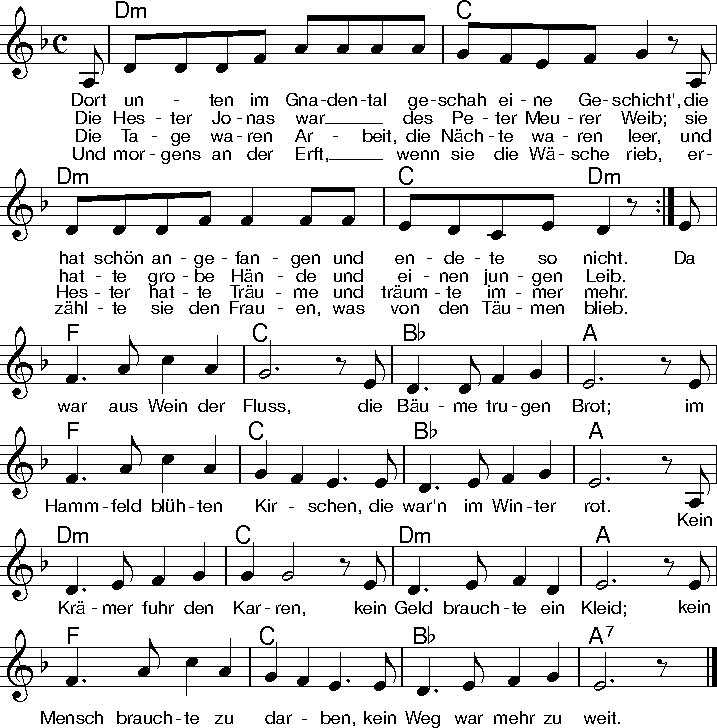
\includegraphics[width=1\textwidth]{Noten/Lied049x.pdf}	

\beginverse
Die \[Dm]Frauen hörten sie mit \[C]lachendem Gesicht;
schön \[Dm]waren Hesters Träume und \[C]schadeten doch \[Dm]nicht. 
Und \[Dm]mittags auf dem Markt, \[C]wo mancher Händler rief,
ge\[Dm]schah, dass um die Jonas mehr \[C]Volk zusammen\[Dm]lief. \newpage
Die \[Dm]Männer zeigten ihr oft \[C]einen schiefen Mund. 
Die \[Dm]besser'n sagten: ''Hester, du \[C]richtest dich zu\[Dm]grund'.''
Des \[Dm]Nachts zum kühlen Gras ka\[C]men sie hungrig doch  
und \[Dm]wollten Hesters Träume und \[C]baten: ''Heute \[Dm]noch.''
\endverse

\beginchorus
Die \[F]Städte werden \[C]fall'n, wo \[Bb]reich nur wenig \[A]sind; 
die \[F]armen Leute \[C]steigen zum \[Bb]Reichtum ohne \[A7]Sünd'.
Und \[Dm]gibt nicht mehr \[C]den Fürst, nicht \[Dm]Bischof und den \[A]Zar 
und \[F]wird nichts sein am \[C]Morgen, wie \[Bb]es am Abend \[A7]war.
\endchorus

\beginverse
Da ^kamen in der Früh' zwei ^Männer aus der Stadt 
und ^schleppten Hester Jonas vor ^einen Magis^trat. 
Da ^war die Red' von Gott, ^da war die Red' von ihr,
da ^war die Red' von Träumen, die ^kränken Mensch und ^Tier.
Und ^quetschten ihr den Hals und ^brachen ihr Gebein;
die ^ganze Stadt hat Tage voll ^Hester Jonas' ^Schrei'n.
Und ^unterschrieb die Schuld mit ^der verkrümmten Hand 
und ^schrie noch lange Träume, bis ^sie das Feuer ^fand.
\endverse
\renewcommand{\everychorus}{\textnote{\bf Refrain (wdh.)}}
%\beginchorus
%\endchorus

\beginverse
Dort \[Dm]unten im Gnadental ge\[C]schah eine Geschicht', 
die \[Dm]hat schön angefangen und \[C]endete so \[Dm]nicht...
\endverse

\endsong

%\beginscripture{}
%Die sogenannte Hexe von Neuss (Ort bei Düsseldorf) - geboren um 1570 - wurde wegen massiven öffentlichen Gerüchten verhaftet und verhört. Man warf der Hebamme und Kräuterheilkundlerin Schadenzauber, den Abfall von Gott und einen Pakt mit dem Teufel vor, was die Hester nach brutaler Folter auch bestätigte. Nach zwischenzeitlicher Flucht wurde sie am 24. Dezember 1935 enthauptet.
%\endscripture
